\documentclass{article}

\usepackage[margin=1in]{geometry}
\usepackage{graphicx}

\title{The Gentrification of the San Francisco Bay Area}
\author{Benicio Bailey, Jacob Feenstra, Diane Kim, Aryan Sarda}

\begin{document}
\maketitle

\section{Introduction}

The San Francisco Bay Area is a vibrant region of our great country, and one of the most economically fertile metropolitan areas in the entire world. It is also the source of arguably the worst gentrification and housing shortage in the United States of America, outstripping even places such as Manhattan and Los Angeles, in housing costs and socioeconomic disparity. 

Gentrification is complex, and while there is no scholarly consensus on it's exact definition, it is generally understood as the process of wealthier individuals moving into lower-income neighborhoods, causing displacement of local residents, increased property value, costlier rents, and a shift in community culture. Indelibly, this leads to a housing shortage, as the cost of buying a home becomes too unaffordable for median income buyers. In the case of the Bay Area, this shortage is vast. The presence of these phenomena in the bay have a shared cause: Silicon Valley.

Technological innovation around the world, and the computer science industry at large, can be traced back to Silicon Valley in the Bay Area. Indeed, it is still the greatest tech hub in the world. Although this is a source of great pride, it is also the predominant cause of gentrification in the Bay Area, as highly paid engineers oust the local residents from the market. As such, as of 2025, it is the most expensive place to live in the United States.

This project will aim to tell the story of gentrification in the Bay Area via an advanced user-led visualization, enabling the users to interactively explore a map of the Bay Area and view gentrification statistics in various parts of the region. The dataset in question consists of six attributes: Population, Median Household Income, Median Home Value, Gross Rent, Vacancy Rate, and Educational Attainment. The last five attributes quantitatively define gentrification; variances in these values, over time, can tell a researcher if regions are gentrified, or \textit{becoming} gentrified. Population will also indicate how gentrification has displaced residents. The dataset is from the American Community Survey census, and dates from 2010 to 2023. With this data, the visualization will map how gentrification has changed over the years. To further corroborate these changes, annotations will be included-- as a timeline-- to timestamp when major changes in Silicon Valley, the Bay Area, or the CS industry in general occurred. 

\section{Our Advanced Visualization}

\begin{figure}[h!]
    \centering
    \begin{minipage}{0.48\textwidth}
        \centering
        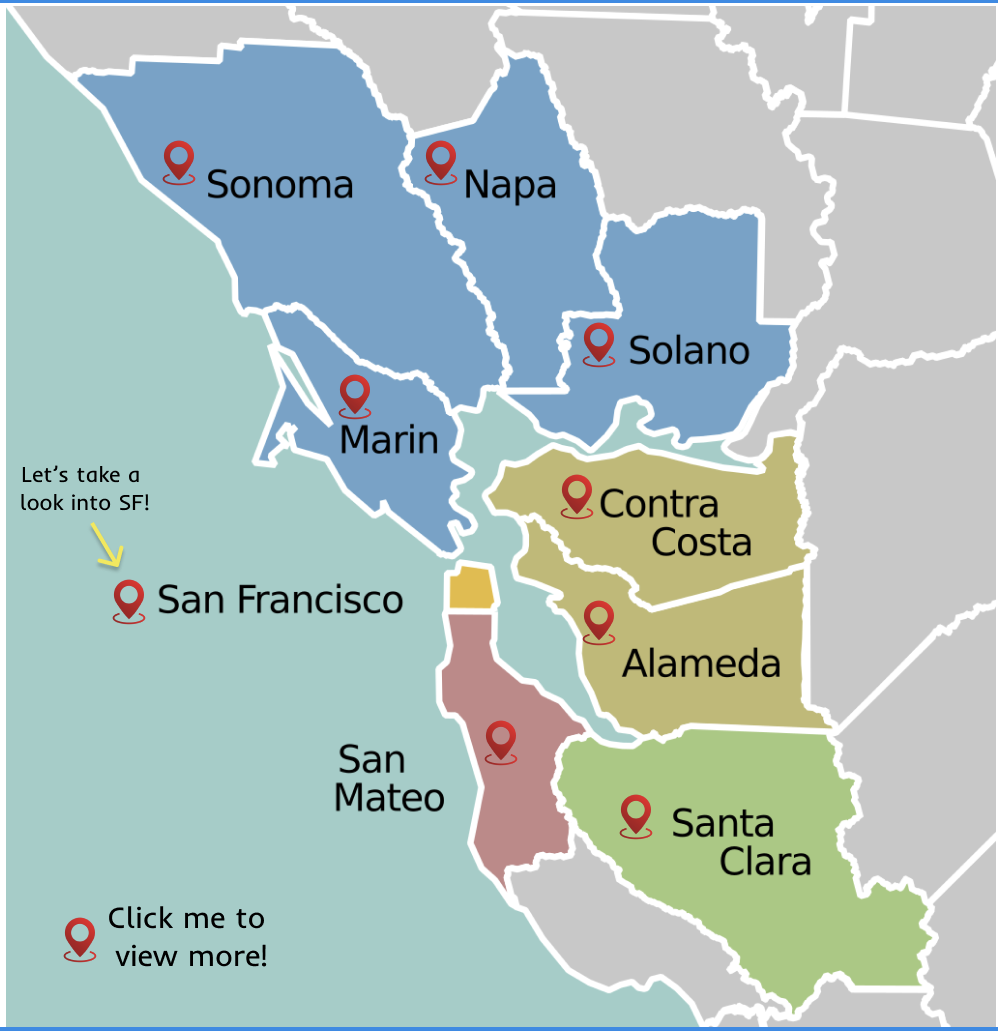
\includegraphics[width=\linewidth]{figure_1.png}
        \caption{View of the Bay Area}
        \label{fig:first}
    \end{minipage}\hfill 
    \begin{minipage}{0.48\textwidth}
        \centering
        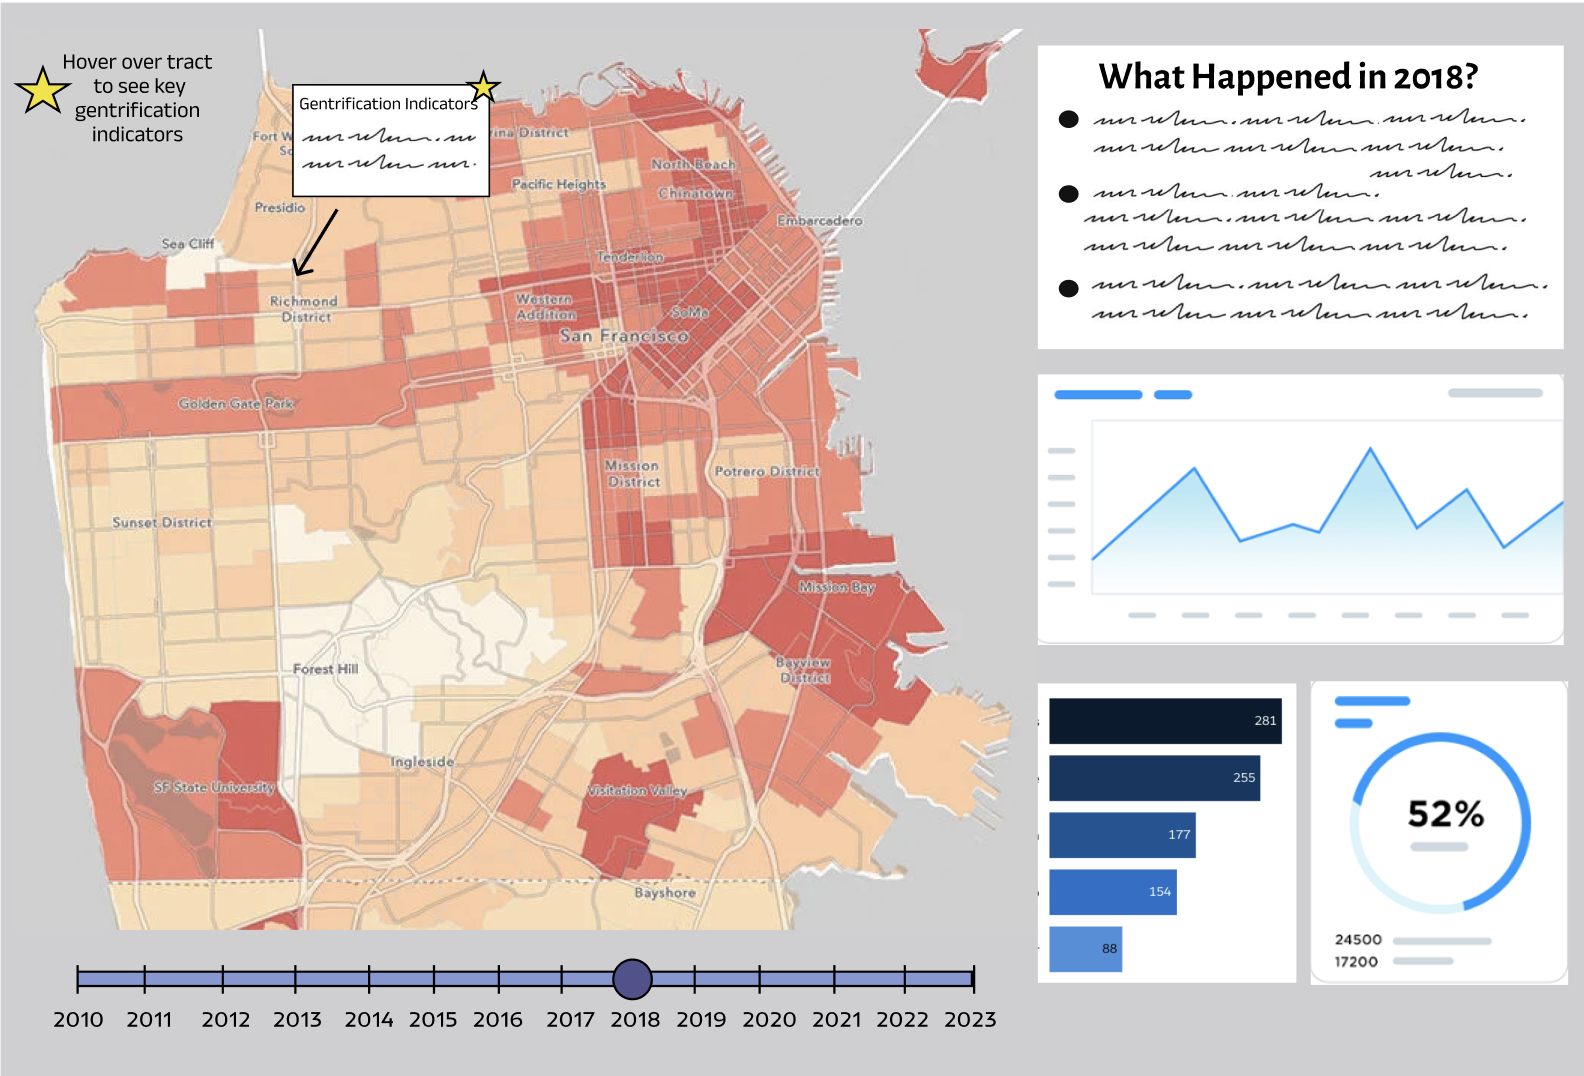
\includegraphics[width=\linewidth]{figure_2.png}
        \caption{View of San Francisco County, by census tract}
        \label{fig:second}
    \end{minipage}
    \caption{Drill-Down approach to explore Bay Area counties}
    \label{fig:combined}
\end{figure}

The visual representation will be a geographic, drill-down map of the San Francisco Bay Area, encompassing the 9 counties within its confines: Alameda, Contra Costa, Marin, Napa, San Francisco, San Mateo, Santa Clara, Solano, and Sonoma (see Figure 1). The outermost view of the Bay Area will include these 9 counties, with larger points of interest (cities, and other relevant locations: we hope to use a GeoJSON as a graphical overlay, which isn't depicted here). The user can interact with one of these counties, and the entire view-space will be occupied by this county, and it's census tracts (see Figure 2). The census tracts will be heatmapped on a color scale; the scale will indicate the magnitude of gentrification for each census tract. It will also serve to distinguish if it is in danger of becoming gentrified, using different colors to do so. A timeline slider will allow the user to step through 2010-2023, indicating how gentrification parameters change, as the heatmap changes.

This county view will be overlaid with a dashboard containing other visualizations (bar charts, and other primitive visualization methods for county-wide averages and insights), and narrative-oriented annotations for the given position in the timeline (namely, what happened that corroborates causes of gentrification in that year, especially with respect to Silicon Valley). These annotations will be contained in a bullet-pointed section. Tooltipping will also be applied when a user hovers over a census tract, showing the gentrification criteria for that tract for the given year (see Figure 3). Note this is subject to moderate changes as we formalize how best to visually tell the story of gentrification.

\section{How The Story Is Told}

The storytelling medium will be a drill-down structure. The firm belief of this project is that the best way to tell the story of gentrification is through user interaction. The user will be able to jump around in timeline and geographical location, constructing the story for themselves, putting the pieces together and noting the trends which will be clearly indicated. While it will be obvious at any point in time what the visualization is conveying, the order of operations in which the user explores these components will be left entirely up to them. The timeline nature of the county view will support a linear approach, but giving complete navigational control to the viewer allows them to focus on particular areas or time periods of interest. It is the belief of this team that the drill-down structure best facilitates this kind of interaction. 

A legend, and cursory explanation of gentrification \& the Bay Area housing shortage, will be shown in the outermost view of the map. The user will then be suggested to click on a county and explore how gentrification has affected it from 2010-2023, and how the housing shortage has changed during these years. The timeline functionality will be front-and-center in this view, and the user will be orientated by the dashboard data and annotations changing as the timeline is interacted with. Gentrification criteria will be "shifting in real-time." The user can understand the cause \& effect of these shifts by pausing to inspect the causal annotations. All transitions, and context, will be self-contained in the visualization as the timeline changes, and the user can take it as slowly as they'd like. It would then be trivial for the user to exit, and visit another county if desired, to repeat the process.

Team 17 is looking forward to delivering this project, and we hope that our visualization sheds light on an issue that is oftentimes abstract \& complicated, and impacts many Californians. Thank you!

\nocite{*}
\bibliographystyle{alpha}
\bibliography{refs}

\end{document}